\documentclass[english]{tktltiki}
\usepackage[pdftex]{graphicx}
\usepackage{subfigure}
\usepackage{url}
\usepackage{tabu}
\begin{document}
\onehalfspacing

\title{Assignment 4: Social computing}
\author{P�ter Ivanics}
\date{\today}

\maketitle

\numberofpagesinformation{\numberofpages\ pages + \numberofappendixpages\ appendices}
\keywords{}

\mytableofcontents

\section{Introduction and background}
	This report compares the nature of users' communication in the official Formula 1 Facebook \cite{F1F} and Instagram \cite{F1I} pages. The report is rolled out as one of the assignment of the Human-Computer Interaction course and serves the purpose to gain hands-on experience with the course material. 
	
	The reason behind choosing the channels of Formula 1 are the popularity of the sport, the recent ending of the 2016 season, as well as my personal interest. The main basis of comparison are the dimensions of computer-mediated communication. The report is carried out from the point of some of the listed dimensions in the original assignment. The analyzed dimensions are introduced in the chapter to follow. 
	
	Before beginning the analysis, let us introduce the official Formula 1 Facebook \cite{F1F} and Instagram \cite{F1I} pages. The two channels are operated by officials and their content is updated fairly regularly during the Formula 1 seasons. In particular, on race weekends this means multiple posts on both channels which often share the same content. Each page has more than 1.9 million followers. These channels are good candidate for this assignment as they represent a sport, are certified, publicly available and have many followers all around the world. 
	
	The 2016 Formula 1 world champion title was decided on the last race of the season last week. Nico Rosberg started the weekend as the championship leader and had to finish at least third on the race to secure the title. Lewis Hamilton still had the chance to claim the title in certain scenarios. This fact makes it interesting to take a look at the activity on the channels of the sport now as a retrospective analysis.
	
	Typically the end of the season brings excitement not only in the champion's title, but also the retiring and freshly signed drivers, who will enter their rookie year in the upcoming season. For example, this year two "veteran" drivers are retiring from the sport which certainly creates discussions in the social media on top of the title battle. Last, but not least there may be other discussion topics, such as next year's new rules, tires, regulations, budget, teams and so on.	
	
\section{Dimensions and hypotheses}
	To begin the analysis with, the dimensions to focus on are chosen. The dimensions used for the analysis in the order of their importance and their descriptions are, as follows.
	
	\begin{enumerate}
		\item Content: what is in the content of the replies to the original post? How do users react to the parent post and what content do they embed in their replies. For instance, smileys, emojis, hashtags, tags of other users, animated images, audiovisual material etc.
		\item Format: the communication is pictorial/textual/based on some other format
		\item Length: System allows short or long messages.
		\item Identity: the communication is anonymous / based on avatar or nickname / with participants' true identity
		\item Messages vs. streams: Communication is message-based vs. a continuous stream
		\item Symmetricity: Communication is the symmetric or asymmetric (i.e., participants do not have equal communication possibilities, e.g. question-and-answer role)
	\end{enumerate}
	
	The first chosen dimension is the content of the replies to the posts. This dimension is chosen because of the hypothesis that the content of the replies on Instagram and Facebook differs in some way. Mainly I expect that the replies on Instagram will include more hashtags in comparison to replies on Facebook, because typically users tend to use this feature intensively on Instagram typically. 
	
	On top of that, I would expect that Instagram users will keep their replies shorter as the application is mainly used from mobile devices while Facebook pages may be visited from desktop devices as well. As it is inconvenient for most people to type extensive text on a touchscreen, the comments under an Instagram post are expected to be shorted and facilitated with user tags and hashtags. Finally, I expect most of the comments to be written in English language on both channels, but some might appear in a foreign language. 
	
\section{Analysis}	
	To begin with, I looked up the first post from each channel in which it was announced, that Nico Rosberg has won the 2016 championship season. Both posts were published on $27^{th}$ November, right after the race in Abu Dhabi ended. Lewis Hamilton has won the race, but Rosberg has finished second and claimed his first-ever F1 champion title.
	
	\begin{figure}[h] 
		\begin{center}
			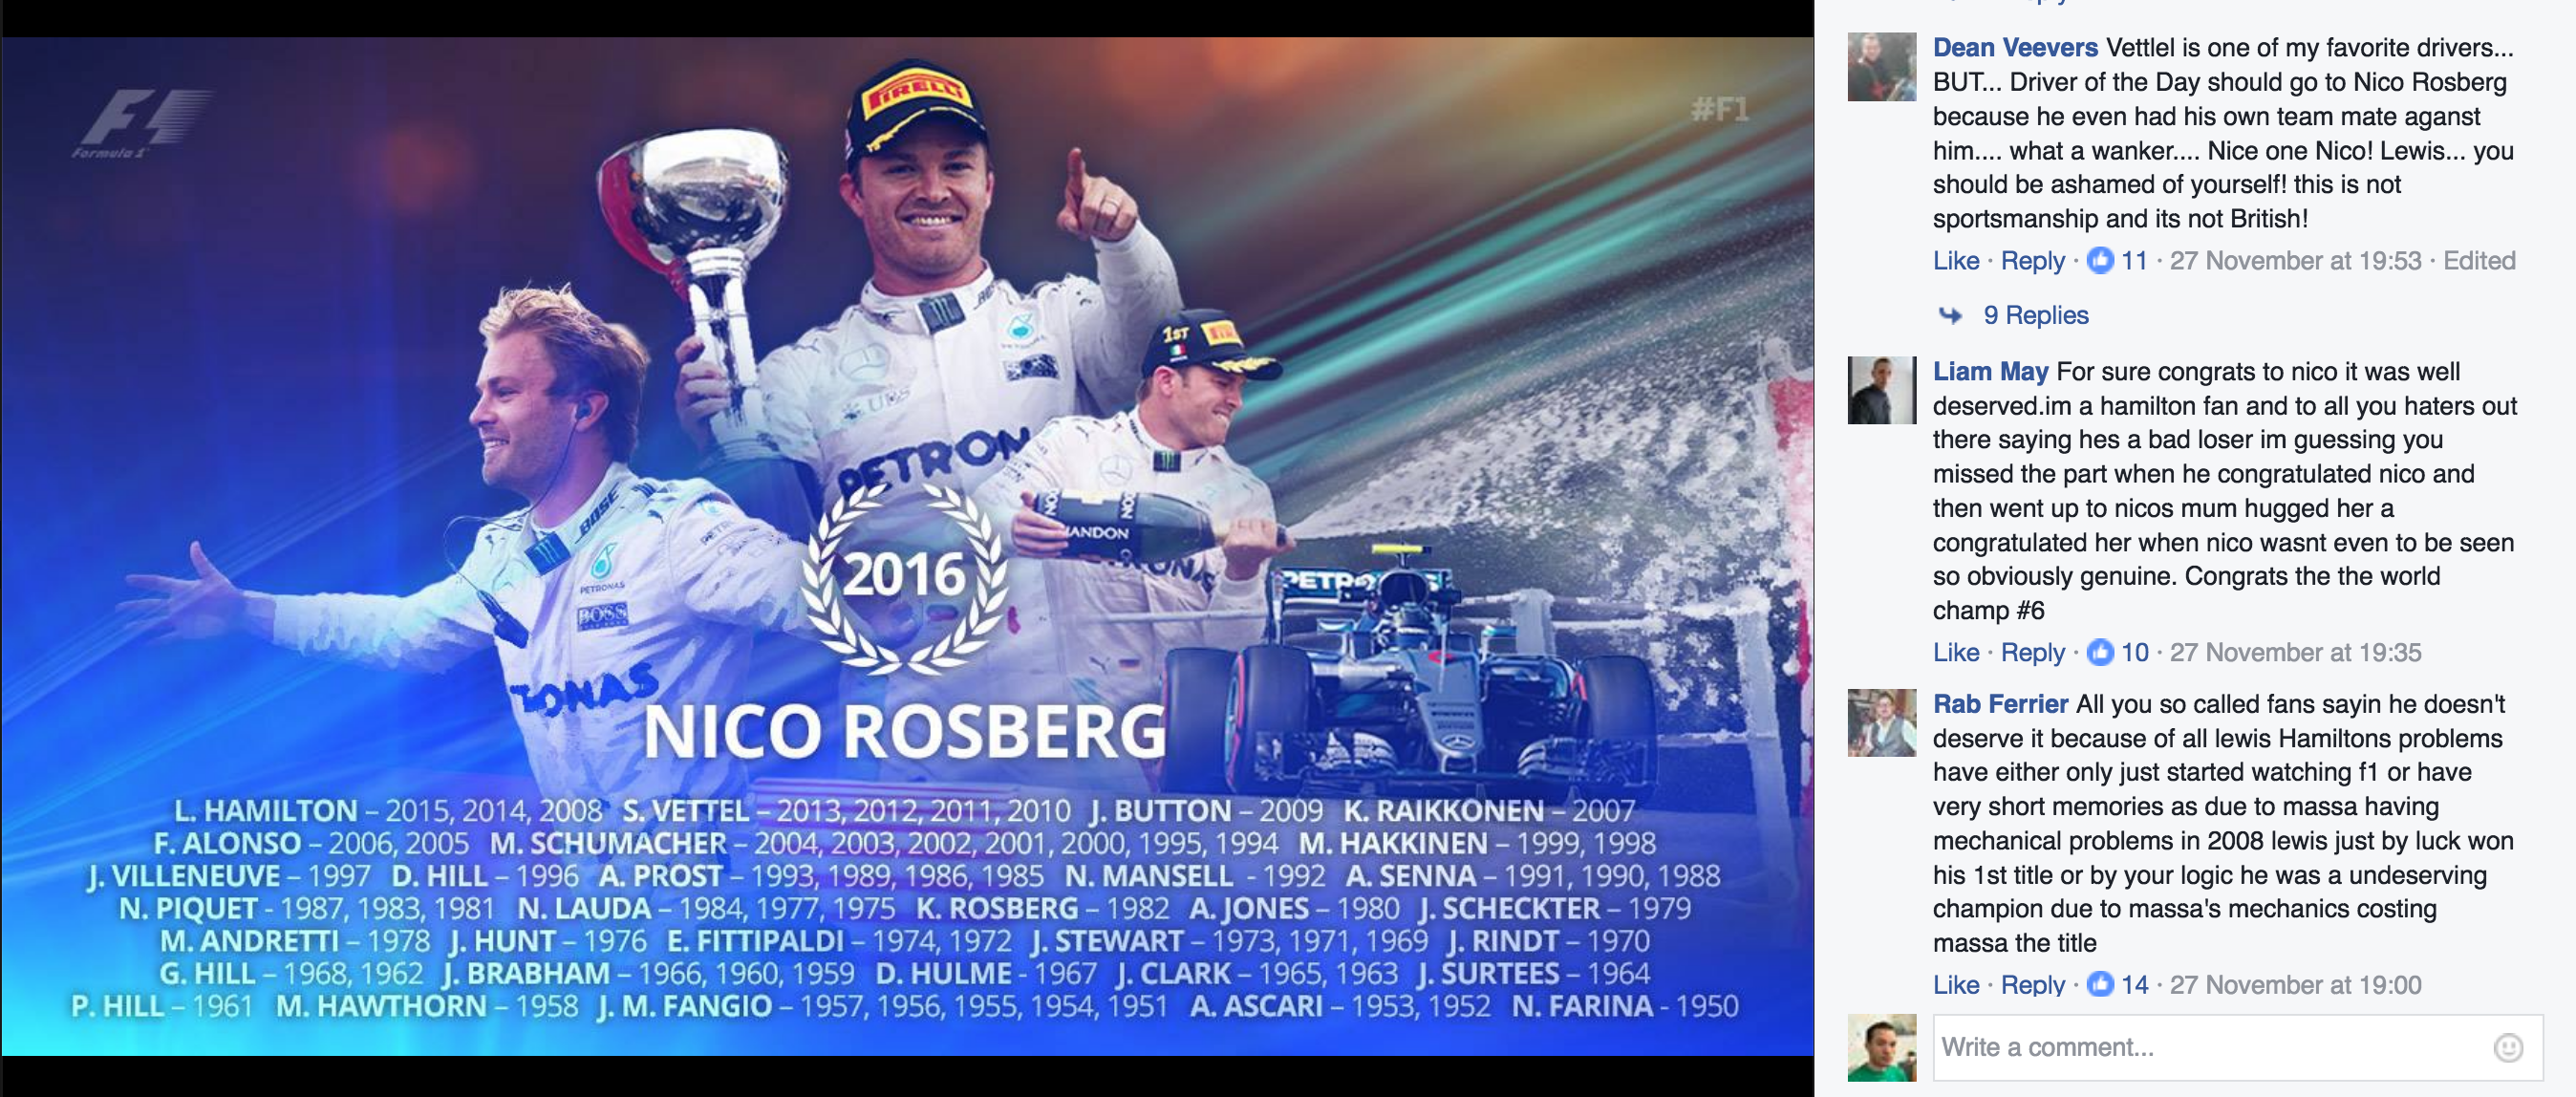
\includegraphics[width=0.9\textwidth]{images/rosberg_f1_wc_facebook.png}
			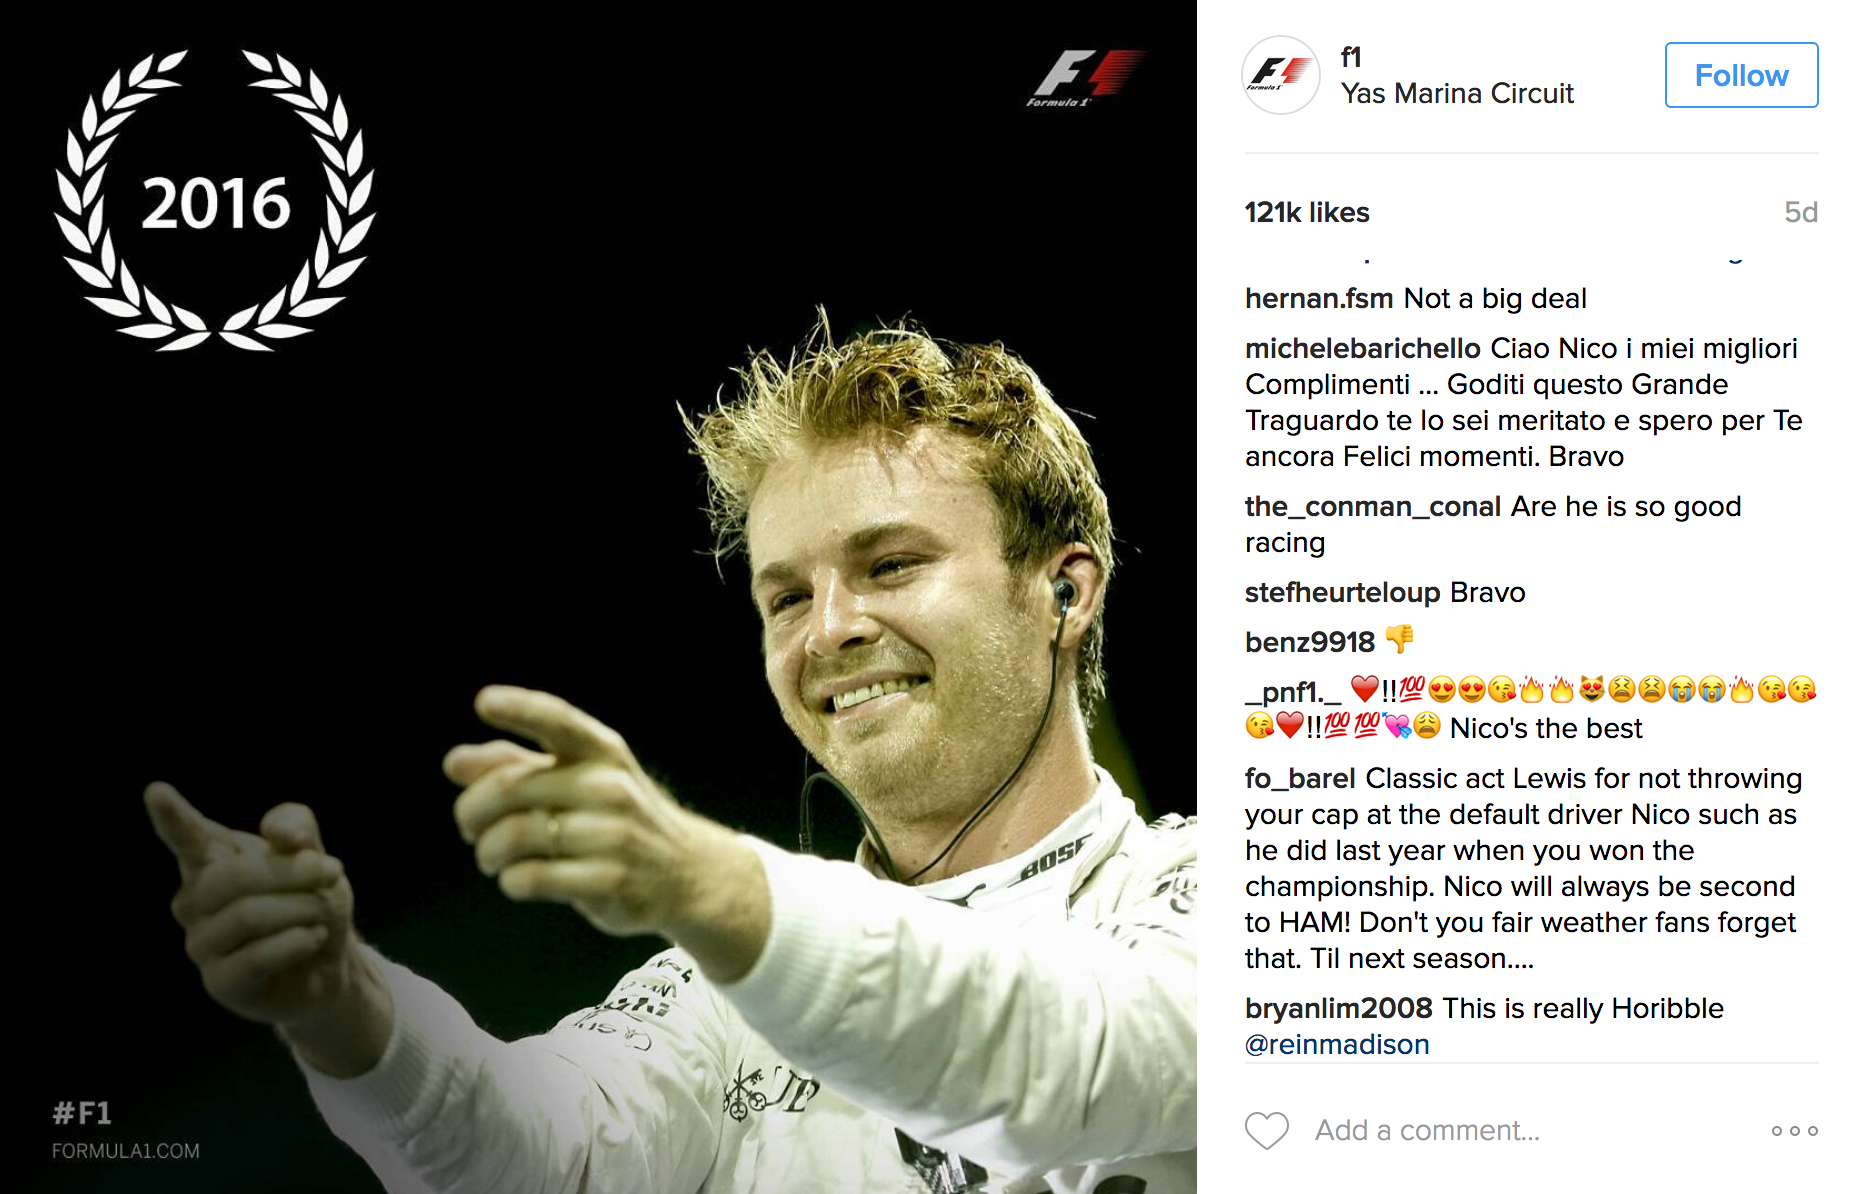
\includegraphics[width=0.9\textwidth]{images/rosberg_f1_wc_instagram.png}
			\caption{A screenshot from the post announcing Nico Rosberg as 2016 Formula 1 world champion from Formula 1's Facebook (top) and Instagram (bottom) pages.}
			\label{rosberg_f1_wc}
		\end{center}
	\end{figure}	
	
	My first observation is that the length of the comments is indeed longer on the Facebook page, while the Instagram users tend to keep their replies rather short. Naturally, many of the users congratulated Nico and Mercedes for claiming the title on both channels, while some Hamilton-fans started flaming and expressed their dislike about the results. 
	
	One interesting finding was that users on Instagram express their opinion rather strong. For instance, one comment referred to Nico as \textit{"Midfield driver"}, another said \textit{"Worst driver of the grid became a WC"}. In comparison, Facebook users expressed their opinion in more lengthy comments in a more "educated" manner, congratulated Nico and reflected on the race as such. Some Facebook users described why they believed Hamilton (or somebody else from the field) is a better driver, while still giving respect to the new champion. Two interesting subsets of the comments is displayed on Figure \ref{rosberg_f1_wc}. While browsing through the comments on the Facebook page, I did not find so offensive comments as the quoted ones above from Instagram. 
	
	Secondly, the hypothesis concerning the usage of emojis, hashtags and user tags in the Instagram comments seemed to be false. I did not see too many of these in any of the channels and it seems users do not use these features it in general. According to my observations, Instagram users tend to attach slightly more smileys/emojis to their comments. This can be related to the short replies as the emojis can express feelings and replace any characters with a proper image. 
	
	Finally, the hypothesis concerning the language of the answers seemed to be correct. On both pages I noticed couple of comments in German, Russian and Spanish. Afterall, there is no surprise in the number of German replies as Nico is originally German and obviously has a lot of fans from his own country. 
	
	To summarize the analysis, let us take a look at the chosen dimensions for each channels. The classification of the channels is displayed in Table \ref{classification-table}.
	
	\begin{table}
	\centering
	\caption{The classification of the channels based on the selected dimensions. } 
	\label{classification-table}
	\begin{tabu} to \textwidth {XXX}
			\\
           & \textbf{Facebook page} & \textbf{Instagram page} \\ \hline
			\textbf{Content} & Lengthier, more "educated" replies & Fairly many flaming and dislike of the original content of the post \\ \hline
			\textbf{Format} & Textual with smileys/emojis, hashtags and user tags & Textual with smileys/emojis, hashtags and user tags \\ \hline
			\textbf{Length} & No limitation on message length & No limitation on message length \\ \hline
			\textbf{Identity} & Known - users have their real names and profile pictures displayed when commenting. & Not necessarily known - users typically have alias/nicknames rather than real, full names.\\ \hline
			\textbf{Messages vs. streams} & Message-based. Audiovisual material may be attached to the original post and to comments by followers. & Message-based. Audiovisual material may be attached to the original post. \\ \hline
			\textbf{Symmetricity} & Asymmetric & Asymmetric \\ \hline
		\end{tabu}
	\end{table}
	
\section{Conclusions}
	The analysis proved some of the hypotheses right and some of them wrong. There are indeed differences between the two computer mediated channels of the Instagram and Facebook pages of Formula 1. The main finding is that the comments under an image in Instagram are tend to be shorter and more facilitated with emojis compared to Facebook replies. On top of that, users on the former channel are more "arrogant" in this particular case. 
	
	As a future research topic it would be interesting to dig deeper into the comments and analyze them in more detail. Furthermore, it would be interesting to take a look at pages of individual drivers or other, similar spots if there is a tendency between users' behavior and in what ways they use these communication channels. 

\nocite{*}
\bibliographystyle{tktl}
\bibliography{bibliography}

\lastpage

\end{document}